\documentclass[]{article}
\usepackage{lmodern}
\usepackage{amssymb,amsmath}
\usepackage{ifxetex,ifluatex}
\usepackage{fixltx2e} % provides \textsubscript
\ifnum 0\ifxetex 1\fi\ifluatex 1\fi=0 % if pdftex
  \usepackage[T1]{fontenc}
  \usepackage[utf8]{inputenc}
\else % if luatex or xelatex
  \ifxetex
    \usepackage{mathspec}
    \usepackage{xltxtra,xunicode}
  \else
    \usepackage{fontspec}
  \fi
  \defaultfontfeatures{Mapping=tex-text,Scale=MatchLowercase}
  \newcommand{\euro}{€}
\fi
% use upquote if available, for straight quotes in verbatim environments
\IfFileExists{upquote.sty}{\usepackage{upquote}}{}
% use microtype if available
\IfFileExists{microtype.sty}{%
\usepackage{microtype}
\UseMicrotypeSet[protrusion]{basicmath} % disable protrusion for tt fonts
}{}
\usepackage[margin=1in]{geometry}
\usepackage{color}
\usepackage{fancyvrb}
\newcommand{\VerbBar}{|}
\newcommand{\VERB}{\Verb[commandchars=\\\{\}]}
\DefineVerbatimEnvironment{Highlighting}{Verbatim}{commandchars=\\\{\}}
% Add ',fontsize=\small' for more characters per line
\usepackage{framed}
\definecolor{shadecolor}{RGB}{248,248,248}
\newenvironment{Shaded}{\begin{snugshade}}{\end{snugshade}}
\newcommand{\KeywordTok}[1]{\textcolor[rgb]{0.13,0.29,0.53}{\textbf{{#1}}}}
\newcommand{\DataTypeTok}[1]{\textcolor[rgb]{0.13,0.29,0.53}{{#1}}}
\newcommand{\DecValTok}[1]{\textcolor[rgb]{0.00,0.00,0.81}{{#1}}}
\newcommand{\BaseNTok}[1]{\textcolor[rgb]{0.00,0.00,0.81}{{#1}}}
\newcommand{\FloatTok}[1]{\textcolor[rgb]{0.00,0.00,0.81}{{#1}}}
\newcommand{\CharTok}[1]{\textcolor[rgb]{0.31,0.60,0.02}{{#1}}}
\newcommand{\StringTok}[1]{\textcolor[rgb]{0.31,0.60,0.02}{{#1}}}
\newcommand{\CommentTok}[1]{\textcolor[rgb]{0.56,0.35,0.01}{\textit{{#1}}}}
\newcommand{\OtherTok}[1]{\textcolor[rgb]{0.56,0.35,0.01}{{#1}}}
\newcommand{\AlertTok}[1]{\textcolor[rgb]{0.94,0.16,0.16}{{#1}}}
\newcommand{\FunctionTok}[1]{\textcolor[rgb]{0.00,0.00,0.00}{{#1}}}
\newcommand{\RegionMarkerTok}[1]{{#1}}
\newcommand{\ErrorTok}[1]{\textbf{{#1}}}
\newcommand{\NormalTok}[1]{{#1}}
\usepackage{graphicx}
\makeatletter
\def\maxwidth{\ifdim\Gin@nat@width>\linewidth\linewidth\else\Gin@nat@width\fi}
\def\maxheight{\ifdim\Gin@nat@height>\textheight\textheight\else\Gin@nat@height\fi}
\makeatother
% Scale images if necessary, so that they will not overflow the page
% margins by default, and it is still possible to overwrite the defaults
% using explicit options in \includegraphics[width, height, ...]{}
\setkeys{Gin}{width=\maxwidth,height=\maxheight,keepaspectratio}
\ifxetex
  \usepackage[setpagesize=false, % page size defined by xetex
              unicode=false, % unicode breaks when used with xetex
              xetex]{hyperref}
\else
  \usepackage[unicode=true]{hyperref}
\fi
\hypersetup{breaklinks=true,
            bookmarks=true,
            pdfauthor={},
            pdftitle={},
            colorlinks=true,
            citecolor=blue,
            urlcolor=blue,
            linkcolor=magenta,
            pdfborder={0 0 0}}
\urlstyle{same}  % don't use monospace font for urls
\setlength{\parindent}{0pt}
\setlength{\parskip}{6pt plus 2pt minus 1pt}
\setlength{\emergencystretch}{3em}  % prevent overfull lines
\setcounter{secnumdepth}{0}

%%% Use protect on footnotes to avoid problems with footnotes in titles
\let\rmarkdownfootnote\footnote%
\def\footnote{\protect\rmarkdownfootnote}

%%% Change title format to be more compact
\usepackage{titling}

% Create subtitle command for use in maketitle
\newcommand{\subtitle}[1]{
  \posttitle{
    \begin{center}\large#1\end{center}
    }
}

\setlength{\droptitle}{-2em}
  \title{}
  \pretitle{\vspace{\droptitle}}
  \posttitle{}
  \author{}
  \preauthor{}\postauthor{}
  \date{}
  \predate{}\postdate{}



\begin{document}

\maketitle


\section{Kaggle}\label{kaggle}

\subsubsection{Titanic: Machine Learning from
Disaster}\label{titanic-machine-learning-from-disaster}

\subsubsection{Introduction}\label{introduction}

This repository holds results for the Kaggle competition: Titanic:
Machine Learning from Disaster.

\subsubsection{Data}\label{data}

The datasets were obtained from the Kaggle Titanic Challenge:
\href{https://www.kaggle.com/c/titanic}{Kaggle page}

\begin{itemize}
\itemsep1pt\parskip0pt\parsep0pt
\item
  Training Dataset:
  \href{https://www.kaggle.com/c/titanic-gettingStarted/download/train.csv}{training
  data}
\item
  Testing Dataset:
  \href{https://www.kaggle.com/c/titanic-gettingStarted/download/test.csv}{test
  data}
\end{itemize}

\subsubsection{1. Loading Packages/ Data}\label{loading-packages-data}

\begin{Shaded}
\begin{Highlighting}[]
\NormalTok{for (package in }\KeywordTok{c}\NormalTok{(}\StringTok{'knitr'}\NormalTok{, }\StringTok{'caret'}\NormalTok{, }\StringTok{'randomForest'}\NormalTok{, }\StringTok{'e1071'}\NormalTok{, }\StringTok{'gbm'}\NormalTok{, }\StringTok{'rpart'}\NormalTok{, }\StringTok{'rpart.plot'}\NormalTok{, }\StringTok{'ggplot2'}\NormalTok{, }\StringTok{'gridExtra'}\NormalTok{)) \{}
  
  \NormalTok{if (!}\KeywordTok{require}\NormalTok{(package, }\DataTypeTok{character.only =} \OtherTok{TRUE}\NormalTok{, }\DataTypeTok{quietly =} \OtherTok{FALSE}\NormalTok{)) \{}
    \KeywordTok{install.packages}\NormalTok{(package)}
    \KeywordTok{library}\NormalTok{(package, }\DataTypeTok{character.only =} \OtherTok{TRUE}\NormalTok{)}
  \NormalTok{\}}
  
\NormalTok{\}}

\NormalTok{val_dfname <-}\StringTok{ }\KeywordTok{c}\NormalTok{(}\StringTok{"train.csv"}\NormalTok{, }\StringTok{"test.csv"}\NormalTok{)}
\NormalTok{val_dfpath <-}\StringTok{ }\KeywordTok{paste}\NormalTok{(}\KeywordTok{getwd}\NormalTok{(), }\StringTok{"/data"}\NormalTok{, }\DataTypeTok{sep =} \StringTok{"/"}\NormalTok{)}

\NormalTok{val_dtrawname <-}\StringTok{ }\KeywordTok{c}\NormalTok{(}\StringTok{"data_training.raw"}\NormalTok{, }\StringTok{"data_testing.raw"}\NormalTok{)}
\NormalTok{val_dtname <-}\StringTok{ }\KeywordTok{c}\NormalTok{(}\StringTok{"data_training"}\NormalTok{, }\StringTok{"data_testing"}\NormalTok{)}

\NormalTok{val_dtclass <-}\StringTok{ }\KeywordTok{c}\NormalTok{(}\StringTok{"val_trainclass"}\NormalTok{, }\StringTok{"val_testclass"}\NormalTok{)}

\NormalTok{val_trainclass <-}\StringTok{ }\KeywordTok{c}\NormalTok{(}\StringTok{"integer"}\NormalTok{,   ## PassengerId}
                    \StringTok{"factor"}\NormalTok{,    ## Survived }
                    \StringTok{"factor"}\NormalTok{,    ## Pclass}
                    \StringTok{"character"}\NormalTok{, ## Name}
                    \StringTok{"factor"}\NormalTok{,    ## Sex}
                    \StringTok{"numeric"}\NormalTok{,   ## Age}
                    \StringTok{"integer"}\NormalTok{,   ## SibSp}
                    \StringTok{"integer"}\NormalTok{,   ## Parch}
                    \StringTok{"character"}\NormalTok{, ## Ticket}
                    \StringTok{"numeric"}\NormalTok{,   ## Fare}
                    \StringTok{"character"}\NormalTok{, ## Cabin}
                    \StringTok{"factor"}\NormalTok{)    ## Embarked}

\NormalTok{val_testclass <-}\StringTok{ }\NormalTok{val_trainclass[-}\DecValTok{2}\NormalTok{]}

\NormalTok{for (i in }\DecValTok{1}\NormalTok{:}\KeywordTok{length}\NormalTok{(val_dtrawname))\{}
  
  \KeywordTok{assign}\NormalTok{(val_dtrawname[i], }\KeywordTok{read.csv}\NormalTok{(}\KeywordTok{paste}\NormalTok{(val_dfpath, val_dfname[i], }\DataTypeTok{sep =} \StringTok{"/"}\NormalTok{), }
                                    \DataTypeTok{na.strings =} \KeywordTok{c}\NormalTok{(}\StringTok{"NA"}\NormalTok{, }\StringTok{""}\NormalTok{), }
                                    \DataTypeTok{colClasses =} \KeywordTok{get}\NormalTok{(val_dtclass[i])))}
  
  \KeywordTok{assign}\NormalTok{(val_dtname[i], }\KeywordTok{get}\NormalTok{(val_dtrawname[i]))}
  
\NormalTok{\}}
\end{Highlighting}
\end{Shaded}

\subsubsection{2. Pre-process the Data}\label{pre-process-the-data}

Check the original data:

\begin{Shaded}
\begin{Highlighting}[]
\NormalTok{## dim(data_training.raw)}
\NormalTok{## str(data_training.raw)}
\KeywordTok{summary}\NormalTok{(data_training.raw)}
\end{Highlighting}
\end{Shaded}

\begin{verbatim}
##   PassengerId    Survived Pclass      Name               Sex     
##  Min.   :  1.0   0:549    1:216   Length:891         female:314  
##  1st Qu.:223.5   1:342    2:184   Class :character   male  :577  
##  Median :446.0            3:491   Mode  :character               
##  Mean   :446.0                                                   
##  3rd Qu.:668.5                                                   
##  Max.   :891.0                                                   
##                                                                  
##       Age            SibSp           Parch           Ticket         
##  Min.   : 0.42   Min.   :0.000   Min.   :0.0000   Length:891        
##  1st Qu.:20.12   1st Qu.:0.000   1st Qu.:0.0000   Class :character  
##  Median :28.00   Median :0.000   Median :0.0000   Mode  :character  
##  Mean   :29.70   Mean   :0.523   Mean   :0.3816                     
##  3rd Qu.:38.00   3rd Qu.:1.000   3rd Qu.:0.0000                     
##  Max.   :80.00   Max.   :8.000   Max.   :6.0000                     
##  NA's   :177                                                        
##       Fare           Cabin           Embarked  
##  Min.   :  0.00   Length:891         C   :168  
##  1st Qu.:  7.91   Class :character   Q   : 77  
##  Median : 14.45   Mode  :character   S   :644  
##  Mean   : 32.20                      NA's:  2  
##  3rd Qu.: 31.00                                
##  Max.   :512.33                                
## 
\end{verbatim}

Categorize passengers by `Title', and create new `FamilySize' Variable:

\begin{Shaded}
\begin{Highlighting}[]
\NormalTok{for (i in }\DecValTok{1}\NormalTok{:}\KeywordTok{length}\NormalTok{(val_dtname))\{}
  
  \NormalTok{temp_data <-}\StringTok{ }\KeywordTok{get}\NormalTok{(val_dtname[i])}
  \NormalTok{temp_data[}\StringTok{"Title"}\NormalTok{] <-}\StringTok{ }\OtherTok{NA}
  \NormalTok{temp_data[}\StringTok{"FamilySize"}\NormalTok{] <-}\StringTok{ }\OtherTok{NA}
  
  \NormalTok{for (j in }\DecValTok{1}\NormalTok{:}\KeywordTok{nrow}\NormalTok{(temp_data))\{}
    
    \NormalTok{temp_data[j, }\StringTok{"Title"}\NormalTok{] <-}\StringTok{ }\KeywordTok{strsplit}\NormalTok{(temp_data[j, }\StringTok{"Name"}\NormalTok{], }\DataTypeTok{split=}\StringTok{'[,.]'}\NormalTok{)[[}\DecValTok{1}\NormalTok{]][}\DecValTok{2}\NormalTok{]}
    \NormalTok{temp_data[j, }\StringTok{"FamilySize"}\NormalTok{] <-}\StringTok{ }\NormalTok{temp_data[j, }\StringTok{"SibSp"}\NormalTok{] +}\StringTok{ }\NormalTok{temp_data[j, }\StringTok{"Parch"}\NormalTok{] +}\StringTok{ }\DecValTok{1}
    
  \NormalTok{\}}
  
  \NormalTok{temp_data[temp_data ==}\StringTok{ ""}\NormalTok{] <-}\StringTok{ }\OtherTok{NA}
  
  \NormalTok{temp_data$Title =}\StringTok{ }\KeywordTok{as.character}\NormalTok{(temp_data$Title)}
  \NormalTok{temp_data$FamilySize =}\StringTok{ }\KeywordTok{as.integer}\NormalTok{(temp_data$FamilySize)}
  \NormalTok{## print(sum(is.na(temp_data$Title)))}
  \NormalTok{## print(sum(is.na(temp_data$FamilySize)))}
  \KeywordTok{assign}\NormalTok{(val_dtname[i], temp_data)}
  
\NormalTok{\}}

\KeywordTok{rm}\NormalTok{(temp_data)}
\end{Highlighting}
\end{Shaded}

Replace NA values within numeric class columns with mean and NA values
within other class columns with most common occurrence:

\begin{Shaded}
\begin{Highlighting}[]
\NormalTok{for (i in }\DecValTok{1}\NormalTok{:}\KeywordTok{length}\NormalTok{(val_dtname))\{}
  
  \NormalTok{temp_data <-}\StringTok{ }\KeywordTok{get}\NormalTok{(val_dtname[i])}
  
  \NormalTok{for (j in }\DecValTok{1}\NormalTok{:}\KeywordTok{ncol}\NormalTok{(temp_data)) \{}
    
    \NormalTok{if (}\KeywordTok{class}\NormalTok{(temp_data[, j]) ==}\StringTok{ "numeric"}\NormalTok{) \{}
      
      \NormalTok{temp_colmean <-}\StringTok{ }\KeywordTok{mean}\NormalTok{(temp_data[, j], }\DataTypeTok{na.rm =} \OtherTok{TRUE}\NormalTok{)}
      \NormalTok{temp_data[, j][}\KeywordTok{which}\NormalTok{(}\KeywordTok{is.na}\NormalTok{(temp_data[, j]))] <-}\StringTok{ }\NormalTok{temp_colmean}
      
    \NormalTok{\} else \{}
      
      \NormalTok{temp_colmode <-}\StringTok{ }\KeywordTok{tail}\NormalTok{(}\KeywordTok{names}\NormalTok{(}\KeywordTok{sort}\NormalTok{(}\KeywordTok{table}\NormalTok{(temp_data[, j]))), }\DecValTok{1}\NormalTok{)}
      \NormalTok{temp_data[, j][}\KeywordTok{which}\NormalTok{(}\KeywordTok{is.na}\NormalTok{(temp_data[, j]))] <-}\StringTok{ }\NormalTok{temp_colmode}

    \NormalTok{\}}
    
  \NormalTok{\}}
   
  \KeywordTok{assign}\NormalTok{(val_dtname[i], temp_data)}

\NormalTok{\}}
  
\KeywordTok{rm}\NormalTok{(temp_data, temp_colmean, temp_colmode)}
\end{Highlighting}
\end{Shaded}

Check the processed data:

\begin{Shaded}
\begin{Highlighting}[]
\NormalTok{## dim(data_training)}
\NormalTok{## str(data_training)}
\KeywordTok{summary}\NormalTok{(data_training)}
\end{Highlighting}
\end{Shaded}

\begin{verbatim}
##  PassengerId        Survived Pclass      Name               Sex     
##  Length:891         0:549    1:216   Length:891         female:314  
##  Class :character   1:342    2:184   Class :character   male  :577  
##  Mode  :character            3:491   Mode  :character               
##                                                                     
##                                                                     
##                                                                     
##       Age           SibSp              Parch              Ticket         
##  Min.   : 0.42   Length:891         Length:891         Length:891        
##  1st Qu.:22.00   Class :character   Class :character   Class :character  
##  Median :29.70   Mode  :character   Mode  :character   Mode  :character  
##  Mean   :29.70                                                           
##  3rd Qu.:35.00                                                           
##  Max.   :80.00                                                           
##       Fare           Cabin           Embarked    Title          
##  Min.   :  0.00   Length:891         C:168    Length:891        
##  1st Qu.:  7.91   Class :character   Q: 77    Class :character  
##  Median : 14.45   Mode  :character   S:646    Mode  :character  
##  Mean   : 32.20                                                 
##  3rd Qu.: 31.00                                                 
##  Max.   :512.33                                                 
##   FamilySize       
##  Length:891        
##  Class :character  
##  Mode  :character  
##                    
##                    
## 
\end{verbatim}

Check the processed data:

\begin{Shaded}
\begin{Highlighting}[]
\NormalTok{tblsumfunc <-}\StringTok{ }\NormalTok{function(x)\{}

  \NormalTok{temp_data <-}\StringTok{ }\KeywordTok{data.frame}\NormalTok{(}\DataTypeTok{Survived =} \NormalTok{data_training$Survived, }\DataTypeTok{Title =} \NormalTok{data_training[[x]], }\DataTypeTok{stringsAsFactors =} \OtherTok{FALSE}\NormalTok{)}
  \NormalTok{temp_obscount <-}\StringTok{ }\KeywordTok{sort}\NormalTok{(}\KeywordTok{table}\NormalTok{(temp_data[, }\DecValTok{2}\NormalTok{]), }\DataTypeTok{decreasing =} \OtherTok{FALSE}\NormalTok{)}
  
  \NormalTok{if (}\KeywordTok{nrow}\NormalTok{(temp_obscount) >}\StringTok{ }\DecValTok{10}\NormalTok{) \{}
    
    \NormalTok{if (}\KeywordTok{class}\NormalTok{(temp_data[, }\DecValTok{2}\NormalTok{]) ==}\StringTok{ "numeric"}\NormalTok{) \{}
      
      \NormalTok{temp_data[, }\DecValTok{2}\NormalTok{] <-}\StringTok{ }\DecValTok{10} \NormalTok{*}\StringTok{ }\KeywordTok{ceiling}\NormalTok{(temp_data[, }\DecValTok{2}\NormalTok{] /}\StringTok{ }\DecValTok{10}\NormalTok{)}
      \NormalTok{## table(temp_data)}
      
    \NormalTok{\} else \{}
    
      \NormalTok{temp_lfobsnm <-}\StringTok{ }\KeywordTok{names}\NormalTok{(temp_obscount[}\DecValTok{1}\NormalTok{:(}\KeywordTok{dim}\NormalTok{(temp_obscount) -}\StringTok{ }\DecValTok{10}\NormalTok{)])}
      \NormalTok{temp_data[, }\DecValTok{2}\NormalTok{][}\KeywordTok{which}\NormalTok{(}\KeywordTok{is.element}\NormalTok{(temp_data[, }\DecValTok{2}\NormalTok{], temp_lfobsnm))] <-}\StringTok{ "Other"}
      \NormalTok{## table(temp_data)}
      
    \NormalTok{\}}
    
  \NormalTok{\}}
  
  \NormalTok{temp_table <-}\StringTok{ }\KeywordTok{table}\NormalTok{(temp_data)}
  \NormalTok{temp_sumtable <-}\StringTok{ }\KeywordTok{addmargins}\NormalTok{(temp_table, }\DataTypeTok{FUN =} \KeywordTok{list}\NormalTok{(}\DataTypeTok{Total =} \NormalTok{sum), }\DataTypeTok{quiet =} \OtherTok{TRUE}\NormalTok{)}
  \NormalTok{temp_proptable <-}\StringTok{ }\KeywordTok{prop.table}\NormalTok{(temp_sumtable[}\KeywordTok{c}\NormalTok{(}\DecValTok{1}\NormalTok{, }\DecValTok{2}\NormalTok{),], }\DecValTok{2}\NormalTok{)}
  \NormalTok{temp_mergedtable <-}\StringTok{ }\KeywordTok{rbind}\NormalTok{(temp_sumtable[}\DecValTok{1}\NormalTok{, ], }
                            \NormalTok{temp_proptable[}\DecValTok{1}\NormalTok{, ], }
                            \NormalTok{temp_sumtable[}\DecValTok{2}\NormalTok{, ], }
                            \NormalTok{temp_proptable[}\DecValTok{2}\NormalTok{, ], }
                            \NormalTok{temp_sumtable[}\DecValTok{3}\NormalTok{, ])}
  \KeywordTok{rownames}\NormalTok{(temp_mergedtable) <-}\StringTok{ }\KeywordTok{c}\NormalTok{(}\StringTok{"Didn't Survive"}\NormalTok{, }\StringTok{"%"}\NormalTok{, }\StringTok{"Survived"}\NormalTok{, }\StringTok{"%"}\NormalTok{, }\StringTok{"Total"}\NormalTok{)}
  
  \KeywordTok{print}\NormalTok{(x)}
  \NormalTok{temp_kabletable <-}\StringTok{ }\KeywordTok{kable}\NormalTok{(temp_mergedtable, }\DataTypeTok{digits =} \DecValTok{2}\NormalTok{, }\DataTypeTok{caption =} \StringTok{"test"}\NormalTok{, }\DataTypeTok{output =} \OtherTok{FALSE}\NormalTok{)}
  \KeywordTok{cat}\NormalTok{(temp_kabletable, }\DataTypeTok{sep=}\StringTok{"}\CharTok{\textbackslash{}n}\StringTok{"}\NormalTok{)}
  \KeywordTok{cat}\NormalTok{(}\DataTypeTok{sep=}\StringTok{"}\CharTok{\textbackslash{}n\textbackslash{}n}\StringTok{"}\NormalTok{)}
  
  \KeywordTok{rm}\NormalTok{(temp_data, temp_table, temp_sumtable, temp_proptable, temp_mergedtable)}
  
\NormalTok{\}}
  
\NormalTok{val_sumcolname <-}\StringTok{ }\KeywordTok{list}\NormalTok{(}\StringTok{"Pclass"}\NormalTok{, }\StringTok{"Title"}\NormalTok{, }\StringTok{"Sex"}\NormalTok{, }\StringTok{"Age"}\NormalTok{, }\StringTok{"FamilySize"}\NormalTok{)}

\NormalTok{for(colname in val_sumcolname) \{ }\KeywordTok{tblsumfunc}\NormalTok{(colname) \}}
\end{Highlighting}
\end{Shaded}

\begin{verbatim}
## [1] "Pclass"
## Table: test
## 
##                        1        2        3    Total
## ---------------  -------  -------  -------  -------
## Didn't Survive     80.00    97.00   372.00   549.00
## %                   0.37     0.53     0.76     0.62
## Survived          136.00    87.00   119.00   342.00
## %                   0.63     0.47     0.24     0.38
## Total             216.00   184.00   491.00   891.00
## 
## [1] "Title"
## Table: test
## 
##                    Col     Dr    Major    Master    Miss    Mlle       Mr      Mrs    Rev    the Countess   Other    Total
## ---------------  -----  -----  -------  --------  ------  ------  -------  -------  -----  --------------  ------  -------
## Didn't Survive     1.0   4.00      1.0     17.00    55.0       0   436.00    26.00      6               0    3.00   549.00
## %                  0.5   0.57      0.5      0.42     0.3       0     0.84     0.21      1               0    0.43     0.62
## Survived           1.0   3.00      1.0     23.00   127.0       2    81.00    99.00      0               1    4.00   342.00
## %                  0.5   0.43      0.5      0.57     0.7       1     0.16     0.79      0               1    0.57     0.38
## Total              2.0   7.00      2.0     40.00   182.0       2   517.00   125.00      6               1    7.00   891.00
## 
## [1] "Sex"
## Table: test
## 
##                   female     male    Total
## ---------------  -------  -------  -------
## Didn't Survive     81.00   468.00   549.00
## %                   0.26     0.81     0.62
## Survived          233.00   109.00   342.00
## %                   0.74     0.19     0.38
## Total             314.00   577.00   891.00
## 
## [1] "Age"
## Table: test
## 
##                      10       20       30       40      50     60      70    80    Total
## ---------------  ------  -------  -------  -------  ------  -----  ------  ----  -------
## Didn't Survive    26.00    71.00   271.00    86.00   53.00   25.0   13.00   4.0   549.00
## %                  0.41     0.62     0.67     0.55    0.62    0.6    0.76   0.8     0.62
## Survived          38.00    44.00   136.00    69.00   33.00   17.0    4.00   1.0   342.00
## %                  0.59     0.38     0.33     0.45    0.38    0.4    0.24   0.2     0.38
## Total             64.00   115.00   407.00   155.00   86.00   42.0   17.00   5.0   891.00
## 
## [1] "FamilySize"
## Table: test
## 
##                       1   11        2        3       4      5       6       7    8    Total
## ---------------  ------  ---  -------  -------  ------  -----  ------  ------  ---  -------
## Didn't Survive    374.0    7    72.00    43.00    8.00   12.0   19.00    8.00    6   549.00
## %                   0.7    1     0.45     0.42    0.28    0.8    0.86    0.67    1     0.62
## Survived          163.0    0    89.00    59.00   21.00    3.0    3.00    4.00    0   342.00
## %                   0.3    0     0.55     0.58    0.72    0.2    0.14    0.33    0     0.38
## Total             537.0    7   161.00   102.00   29.00   15.0   22.00   12.00    6   891.00
\end{verbatim}

At a high level, the data suggests that passengers within the following
groups had an improved survival rate: * Were Class 1 passengers * Had a
title of `Master' / aged 0-10 * Were female * Boarded with a family of
size 2-4

Chart the processed data:

\begin{Shaded}
\begin{Highlighting}[]
\NormalTok{val_agehist <-}\StringTok{ }\KeywordTok{ggplot}\NormalTok{(data_training, }\KeywordTok{aes}\NormalTok{(}\DataTypeTok{x =} \NormalTok{Age, }\DataTypeTok{fill =} \NormalTok{Survived)) +}
\StringTok{                      }\KeywordTok{geom_histogram}\NormalTok{() +}
\StringTok{                      }\KeywordTok{ggtitle}\NormalTok{(}\StringTok{"Age vs Survival"}\NormalTok{) +}
\StringTok{                      }\KeywordTok{theme}\NormalTok{(}\DataTypeTok{legend.position =} \StringTok{"bottom"}\NormalTok{) +}
\StringTok{                      }\KeywordTok{scale_fill_discrete}\NormalTok{(}\DataTypeTok{labels =} \KeywordTok{c}\NormalTok{(}\StringTok{"No"}\NormalTok{, }\StringTok{"Yes"}\NormalTok{))}

\NormalTok{val_sexhist <-}\StringTok{ }\KeywordTok{ggplot}\NormalTok{(data_training, }\KeywordTok{aes}\NormalTok{(}\DataTypeTok{x =} \NormalTok{Sex, }\DataTypeTok{fill =} \NormalTok{Survived)) +}
\StringTok{                      }\KeywordTok{geom_histogram}\NormalTok{() +}
\StringTok{                      }\KeywordTok{ggtitle}\NormalTok{(}\StringTok{"Age vs Survival"}\NormalTok{) +}
\StringTok{                      }\KeywordTok{theme}\NormalTok{(}\DataTypeTok{legend.position =} \StringTok{"bottom"}\NormalTok{) +}
\StringTok{                      }\KeywordTok{scale_fill_discrete}\NormalTok{(}\DataTypeTok{labels =} \KeywordTok{c}\NormalTok{(}\StringTok{"No"}\NormalTok{, }\StringTok{"Yes"}\NormalTok{))}

\KeywordTok{grid.arrange}\NormalTok{(val_agehist, val_sexhist, }\DataTypeTok{ncol =} \DecValTok{2}\NormalTok{)}
\end{Highlighting}
\end{Shaded}

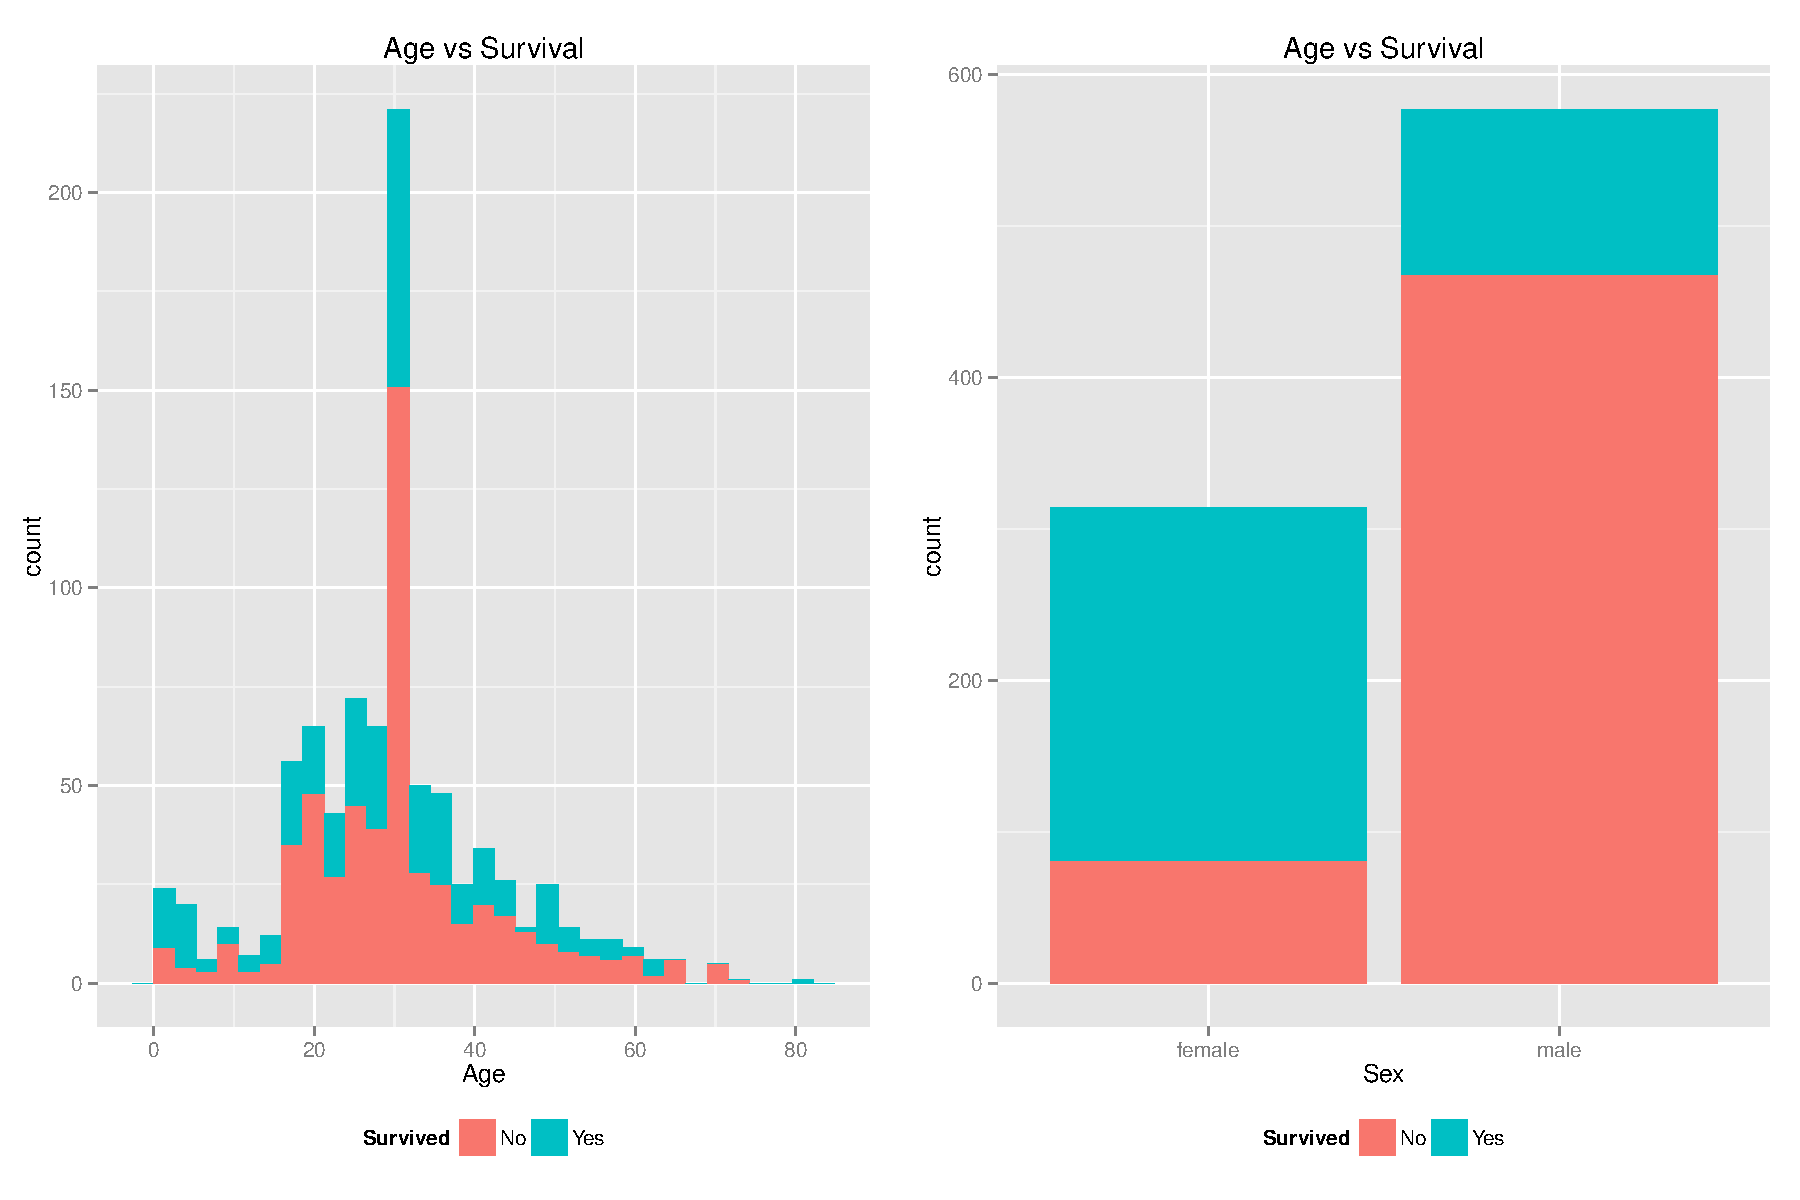
\includegraphics{figure/unnamed-chunk-7-1.pdf}

\begin{Shaded}
\begin{Highlighting}[]
\NormalTok{val_pclasshist <-}\StringTok{ }\KeywordTok{ggplot}\NormalTok{(data_training, }\KeywordTok{aes}\NormalTok{(}\DataTypeTok{x =} \NormalTok{Pclass, }\DataTypeTok{fill =} \NormalTok{Survived)) +}
\StringTok{                        }\KeywordTok{geom_histogram}\NormalTok{() +}
\StringTok{                        }\KeywordTok{ggtitle}\NormalTok{(}\StringTok{"Passenger Class vs Survival"}\NormalTok{) +}
\StringTok{                        }\KeywordTok{theme}\NormalTok{(}\DataTypeTok{legend.position =} \StringTok{"right"}\NormalTok{) +}
\StringTok{                        }\KeywordTok{scale_fill_discrete}\NormalTok{(}\DataTypeTok{labels =} \KeywordTok{c}\NormalTok{(}\StringTok{"No"}\NormalTok{, }\StringTok{"Yes"}\NormalTok{))}

\NormalTok{val_titlehist <-}\StringTok{ }\KeywordTok{ggplot}\NormalTok{(data_training, }\KeywordTok{aes}\NormalTok{(}\DataTypeTok{x =} \NormalTok{Title, }\DataTypeTok{fill =} \NormalTok{Survived)) +}
\StringTok{                        }\KeywordTok{geom_histogram}\NormalTok{() +}
\StringTok{                        }\KeywordTok{ggtitle}\NormalTok{(}\StringTok{"Title vs Survival"}\NormalTok{) +}
\StringTok{                        }\KeywordTok{theme}\NormalTok{(}\DataTypeTok{legend.position =} \StringTok{"right"}\NormalTok{) +}
\StringTok{                        }\KeywordTok{scale_fill_discrete}\NormalTok{(}\DataTypeTok{labels =} \KeywordTok{c}\NormalTok{(}\StringTok{"No"}\NormalTok{, }\StringTok{"Yes"}\NormalTok{))}

\NormalTok{val_familyhist <-}\StringTok{ }\KeywordTok{ggplot}\NormalTok{(data_training, }\KeywordTok{aes}\NormalTok{(}\DataTypeTok{x =} \NormalTok{FamilySize, }\DataTypeTok{fill =} \NormalTok{Survived)) +}
\StringTok{                        }\KeywordTok{geom_histogram}\NormalTok{() +}
\StringTok{                        }\KeywordTok{ggtitle}\NormalTok{(}\StringTok{"Family Size vs Survival"}\NormalTok{) +}
\StringTok{                        }\KeywordTok{theme}\NormalTok{(}\DataTypeTok{legend.position =} \StringTok{"right"}\NormalTok{) +}
\StringTok{                        }\KeywordTok{scale_fill_discrete}\NormalTok{(}\DataTypeTok{labels =} \KeywordTok{c}\NormalTok{(}\StringTok{"No"}\NormalTok{, }\StringTok{"Yes"}\NormalTok{))}

\KeywordTok{grid.arrange}\NormalTok{(val_pclasshist, val_titlehist, val_familyhist, }\DataTypeTok{nrow =} \DecValTok{3}\NormalTok{)}
\end{Highlighting}
\end{Shaded}

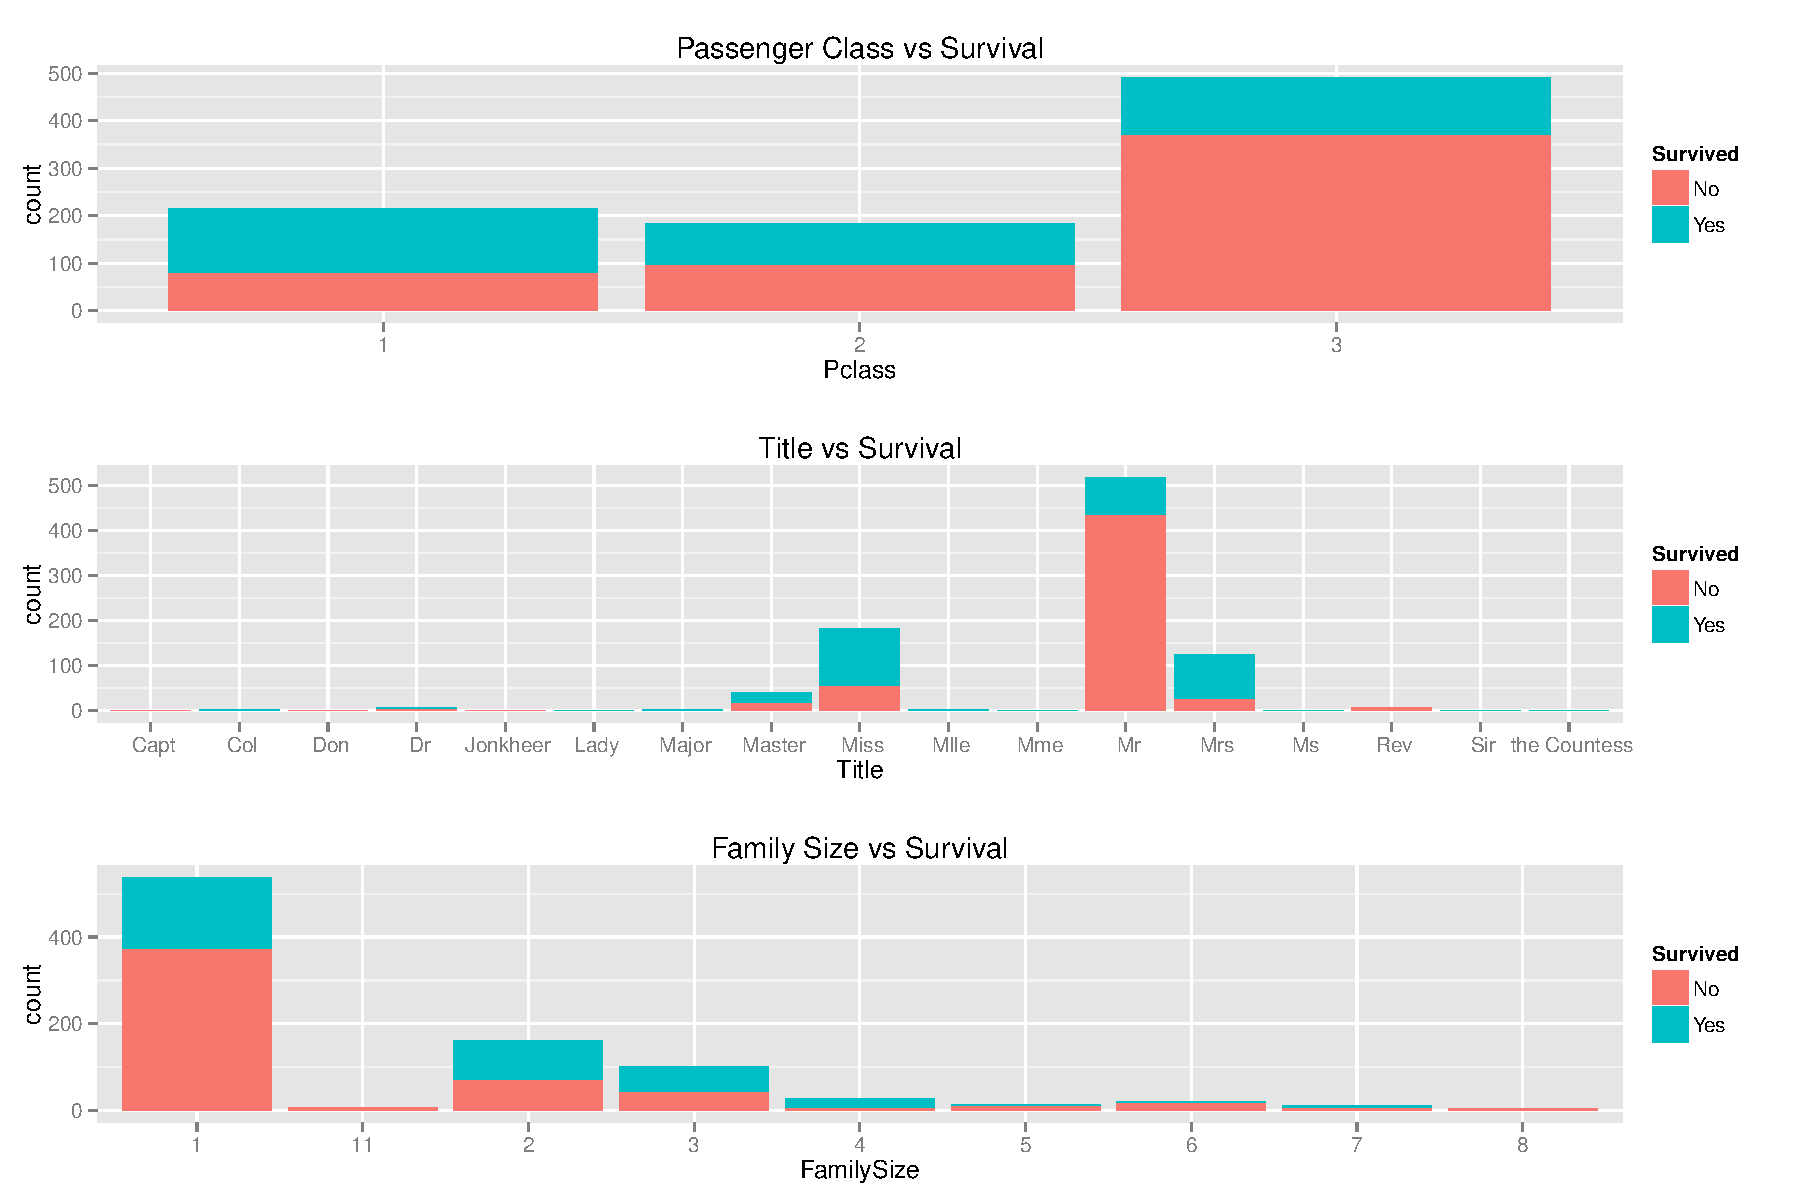
\includegraphics{figure/unnamed-chunk-7-2.pdf}

\subsubsection{3. Prediction Modelling}\label{prediction-modelling}

Split the training data:

\begin{Shaded}
\begin{Highlighting}[]
\KeywordTok{set.seed}\NormalTok{(}\DecValTok{12345}\NormalTok{)}
\NormalTok{data_training.rows <-}\StringTok{ }\KeywordTok{createDataPartition}\NormalTok{(data_training$Survived, }\DataTypeTok{p =} \FloatTok{0.7}\NormalTok{, }\DataTypeTok{list =} \OtherTok{FALSE}\NormalTok{)}

\NormalTok{data_training.train <-}\StringTok{ }\NormalTok{data_training[data_training.rows, ]}
\NormalTok{data_training.test <-}\StringTok{ }\NormalTok{data_training[-data_training.rows, ]}
\end{Highlighting}
\end{Shaded}

Check the split data:

\begin{Shaded}
\begin{Highlighting}[]
\NormalTok{## dim(data_training.train)}
\KeywordTok{str}\NormalTok{(data_training.train)}
\end{Highlighting}
\end{Shaded}

\begin{verbatim}
## 'data.frame':    625 obs. of  14 variables:
##  $ PassengerId: chr  "1" "3" "4" "6" ...
##  $ Survived   : Factor w/ 2 levels "0","1": 1 2 2 1 1 1 2 2 2 1 ...
##  $ Pclass     : Factor w/ 3 levels "1","2","3": 3 3 1 3 1 3 3 2 1 3 ...
##  $ Name       : chr  "Braund, Mr. Owen Harris" "Heikkinen, Miss. Laina" "Futrelle, Mrs. Jacques Heath (Lily May Peel)" "Moran, Mr. James" ...
##  $ Sex        : Factor w/ 2 levels "female","male": 2 1 1 2 2 2 1 1 1 2 ...
##  $ Age        : num  22 26 35 29.7 54 ...
##  $ SibSp      : chr  "1" "0" "1" "0" ...
##  $ Parch      : chr  "0" "0" "0" "0" ...
##  $ Ticket     : chr  "A/5 21171" "STON/O2. 3101282" "113803" "330877" ...
##  $ Fare       : num  7.25 7.92 53.1 8.46 51.86 ...
##  $ Cabin      : chr  "G6" "G6" "C123" "G6" ...
##  $ Embarked   : Factor w/ 3 levels "C","Q","S": 3 3 3 2 3 3 3 1 3 3 ...
##  $ Title      : chr  " Mr" " Miss" " Mrs" " Mr" ...
##  $ FamilySize : chr  "2" "1" "2" "1" ...
\end{verbatim}

\begin{Shaded}
\begin{Highlighting}[]
\NormalTok{## summary(data_training.train)}

\NormalTok{## dim(data_training.test)}
\KeywordTok{str}\NormalTok{(data_training.test)}
\end{Highlighting}
\end{Shaded}

\begin{verbatim}
## 'data.frame':    266 obs. of  14 variables:
##  $ PassengerId: chr  "2" "5" "11" "16" ...
##  $ Survived   : Factor w/ 2 levels "0","1": 2 1 2 2 2 1 1 2 1 2 ...
##  $ Pclass     : Factor w/ 3 levels "1","2","3": 1 3 3 2 3 2 3 3 2 3 ...
##  $ Name       : chr  "Cumings, Mrs. John Bradley (Florence Briggs Thayer)" "Allen, Mr. William Henry" "Sandstrom, Miss. Marguerite Rut" "Hewlett, Mrs. (Mary D Kingcome) " ...
##  $ Sex        : Factor w/ 2 levels "female","male": 1 2 1 1 1 2 1 1 2 2 ...
##  $ Age        : num  38 35 4 55 29.7 ...
##  $ SibSp      : chr  "1" "0" "1" "0" ...
##  $ Parch      : chr  "0" "0" "1" "0" ...
##  $ Ticket     : chr  "PC 17599" "373450" "PP 9549" "248706" ...
##  $ Fare       : num  71.28 8.05 16.7 16 7.22 ...
##  $ Cabin      : chr  "C85" "G6" "G6" "G6" ...
##  $ Embarked   : Factor w/ 3 levels "C","Q","S": 1 3 3 3 1 3 3 3 3 1 ...
##  $ Title      : chr  " Mrs" " Mr" " Miss" " Mrs" ...
##  $ FamilySize : chr  "2" "1" "3" "1" ...
\end{verbatim}

\begin{Shaded}
\begin{Highlighting}[]
\NormalTok{## summary(data_training.test)}
\end{Highlighting}
\end{Shaded}

\paragraph{Decision tree prediction}\label{decision-tree-prediction}

\begin{Shaded}
\begin{Highlighting}[]
\KeywordTok{set.seed}\NormalTok{(}\DecValTok{12345}\NormalTok{)}
\NormalTok{val_dtmodel <-}\StringTok{ }\KeywordTok{rpart}\NormalTok{(Survived ~}\StringTok{ }\NormalTok{Pclass +}\StringTok{ }\NormalTok{Sex +}\StringTok{ }\NormalTok{Age +}\StringTok{ }\NormalTok{Fare +}\StringTok{ }\NormalTok{Embarked +}\StringTok{ }\NormalTok{FamilySize, }\DataTypeTok{data =} \NormalTok{data_training.train, }\DataTypeTok{method =} \StringTok{"class"}\NormalTok{)}
\NormalTok{val_dtmodel.predict <-}\StringTok{ }\KeywordTok{predict}\NormalTok{(val_dtmodel, data_training.test, }\DataTypeTok{type =} \StringTok{"class"}\NormalTok{)}
\NormalTok{val_dtcm <-}\StringTok{ }\KeywordTok{confusionMatrix}\NormalTok{(val_dtmodel.predict, data_training.test$Survived)}
\NormalTok{val_dtcm}
\end{Highlighting}
\end{Shaded}

\begin{verbatim}
## Confusion Matrix and Statistics
## 
##           Reference
## Prediction   0   1
##          0 145  38
##          1  19  64
##                                           
##                Accuracy : 0.7857          
##                  95% CI : (0.7315, 0.8335)
##     No Information Rate : 0.6165          
##     P-Value [Acc > NIR] : 2.603e-09       
##                                           
##                   Kappa : 0.5303          
##  Mcnemar's Test P-Value : 0.01712         
##                                           
##             Sensitivity : 0.8841          
##             Specificity : 0.6275          
##          Pos Pred Value : 0.7923          
##          Neg Pred Value : 0.7711          
##              Prevalence : 0.6165          
##          Detection Rate : 0.5451          
##    Detection Prevalence : 0.6880          
##       Balanced Accuracy : 0.7558          
##                                           
##        'Positive' Class : 0               
## 
\end{verbatim}

Decision tree prediction has a reported accuracy against the training
dataset:

\begin{Shaded}
\begin{Highlighting}[]
\KeywordTok{round}\NormalTok{(val_dtcm$overall[}\StringTok{'Accuracy'}\NormalTok{], }\DecValTok{4}\NormalTok{)}
\end{Highlighting}
\end{Shaded}

\begin{verbatim}
## Accuracy 
##   0.7857
\end{verbatim}

\begin{Shaded}
\begin{Highlighting}[]
\KeywordTok{plot}\NormalTok{(val_dtcm$table, }
    \DataTypeTok{col =} \NormalTok{val_dtcm$byClass, }
    \DataTypeTok{main =} \KeywordTok{paste}\NormalTok{(}\StringTok{"Decision Tree Confusion Matrix: Accuracy ="}\NormalTok{, }
    \KeywordTok{round}\NormalTok{(val_dtcm$overall[}\StringTok{'Accuracy'}\NormalTok{], }\DecValTok{4}\NormalTok{)))}
\end{Highlighting}
\end{Shaded}

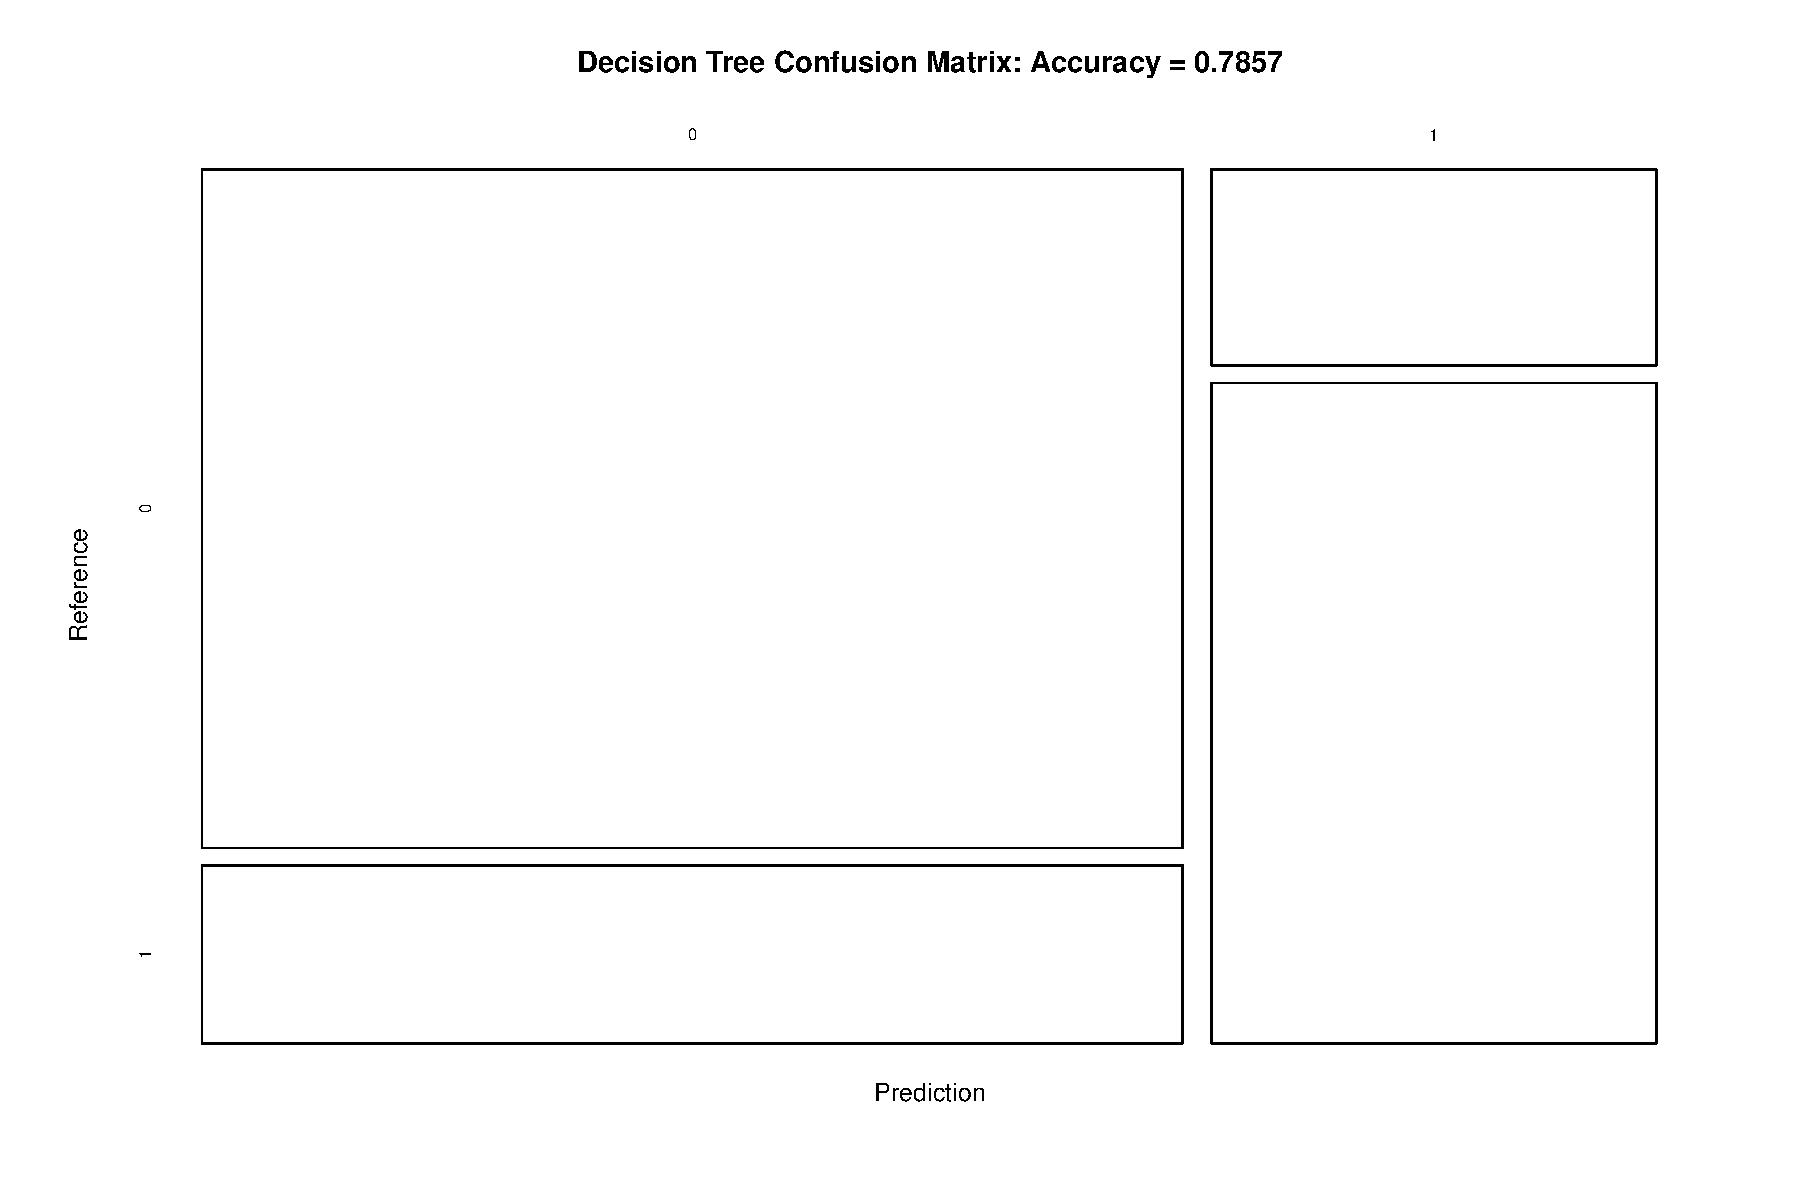
\includegraphics{figure/unnamed-chunk-12-1.pdf}

\paragraph{Random forest prediction}\label{random-forest-prediction}

\begin{Shaded}
\begin{Highlighting}[]
\KeywordTok{set.seed}\NormalTok{(}\DecValTok{12345}\NormalTok{)}
\NormalTok{val_rfmodel <-}\StringTok{ }\KeywordTok{randomForest}\NormalTok{(Survived ~}\StringTok{ }\NormalTok{Pclass +}\StringTok{ }\NormalTok{Sex +}\StringTok{ }\NormalTok{Age +}\StringTok{ }\NormalTok{Fare +}\StringTok{ }\NormalTok{Embarked +}\StringTok{ }\NormalTok{FamilySize, }\DataTypeTok{data =} \NormalTok{data_training.train)}
\NormalTok{val_rfmodel.predict <-}\StringTok{ }\KeywordTok{predict}\NormalTok{(val_rfmodel, data_training.test, }\DataTypeTok{type =} \StringTok{"class"}\NormalTok{)}
\NormalTok{val_rfcm <-}\StringTok{ }\KeywordTok{confusionMatrix}\NormalTok{(val_rfmodel.predict, data_training.test$Survived)}
\NormalTok{val_rfcm}
\end{Highlighting}
\end{Shaded}

\begin{verbatim}
## Confusion Matrix and Statistics
## 
##           Reference
## Prediction   0   1
##          0 149  33
##          1  15  69
##                                          
##                Accuracy : 0.8195         
##                  95% CI : (0.768, 0.8638)
##     No Information Rate : 0.6165         
##     P-Value [Acc > NIR] : 5.675e-13      
##                                          
##                   Kappa : 0.6052         
##  Mcnemar's Test P-Value : 0.01414        
##                                          
##             Sensitivity : 0.9085         
##             Specificity : 0.6765         
##          Pos Pred Value : 0.8187         
##          Neg Pred Value : 0.8214         
##              Prevalence : 0.6165         
##          Detection Rate : 0.5602         
##    Detection Prevalence : 0.6842         
##       Balanced Accuracy : 0.7925         
##                                          
##        'Positive' Class : 0              
## 
\end{verbatim}

Random forest prediction has a reported accuracy against the training
dataset:

\begin{Shaded}
\begin{Highlighting}[]
\KeywordTok{round}\NormalTok{(val_rfcm$overall[}\StringTok{'Accuracy'}\NormalTok{], }\DecValTok{4}\NormalTok{)}
\end{Highlighting}
\end{Shaded}

\begin{verbatim}
## Accuracy 
##   0.8195
\end{verbatim}

\begin{Shaded}
\begin{Highlighting}[]
\KeywordTok{plot}\NormalTok{(val_rfcm$table, }
    \DataTypeTok{col =} \NormalTok{val_rfcm$byClass, }
    \DataTypeTok{main =} \KeywordTok{paste}\NormalTok{(}\StringTok{"Random Forest Confusion Matrix: Accuracy ="}\NormalTok{,}
    \KeywordTok{round}\NormalTok{(val_rfcm$overall[}\StringTok{'Accuracy'}\NormalTok{], }\DecValTok{4}\NormalTok{)))}
\end{Highlighting}
\end{Shaded}

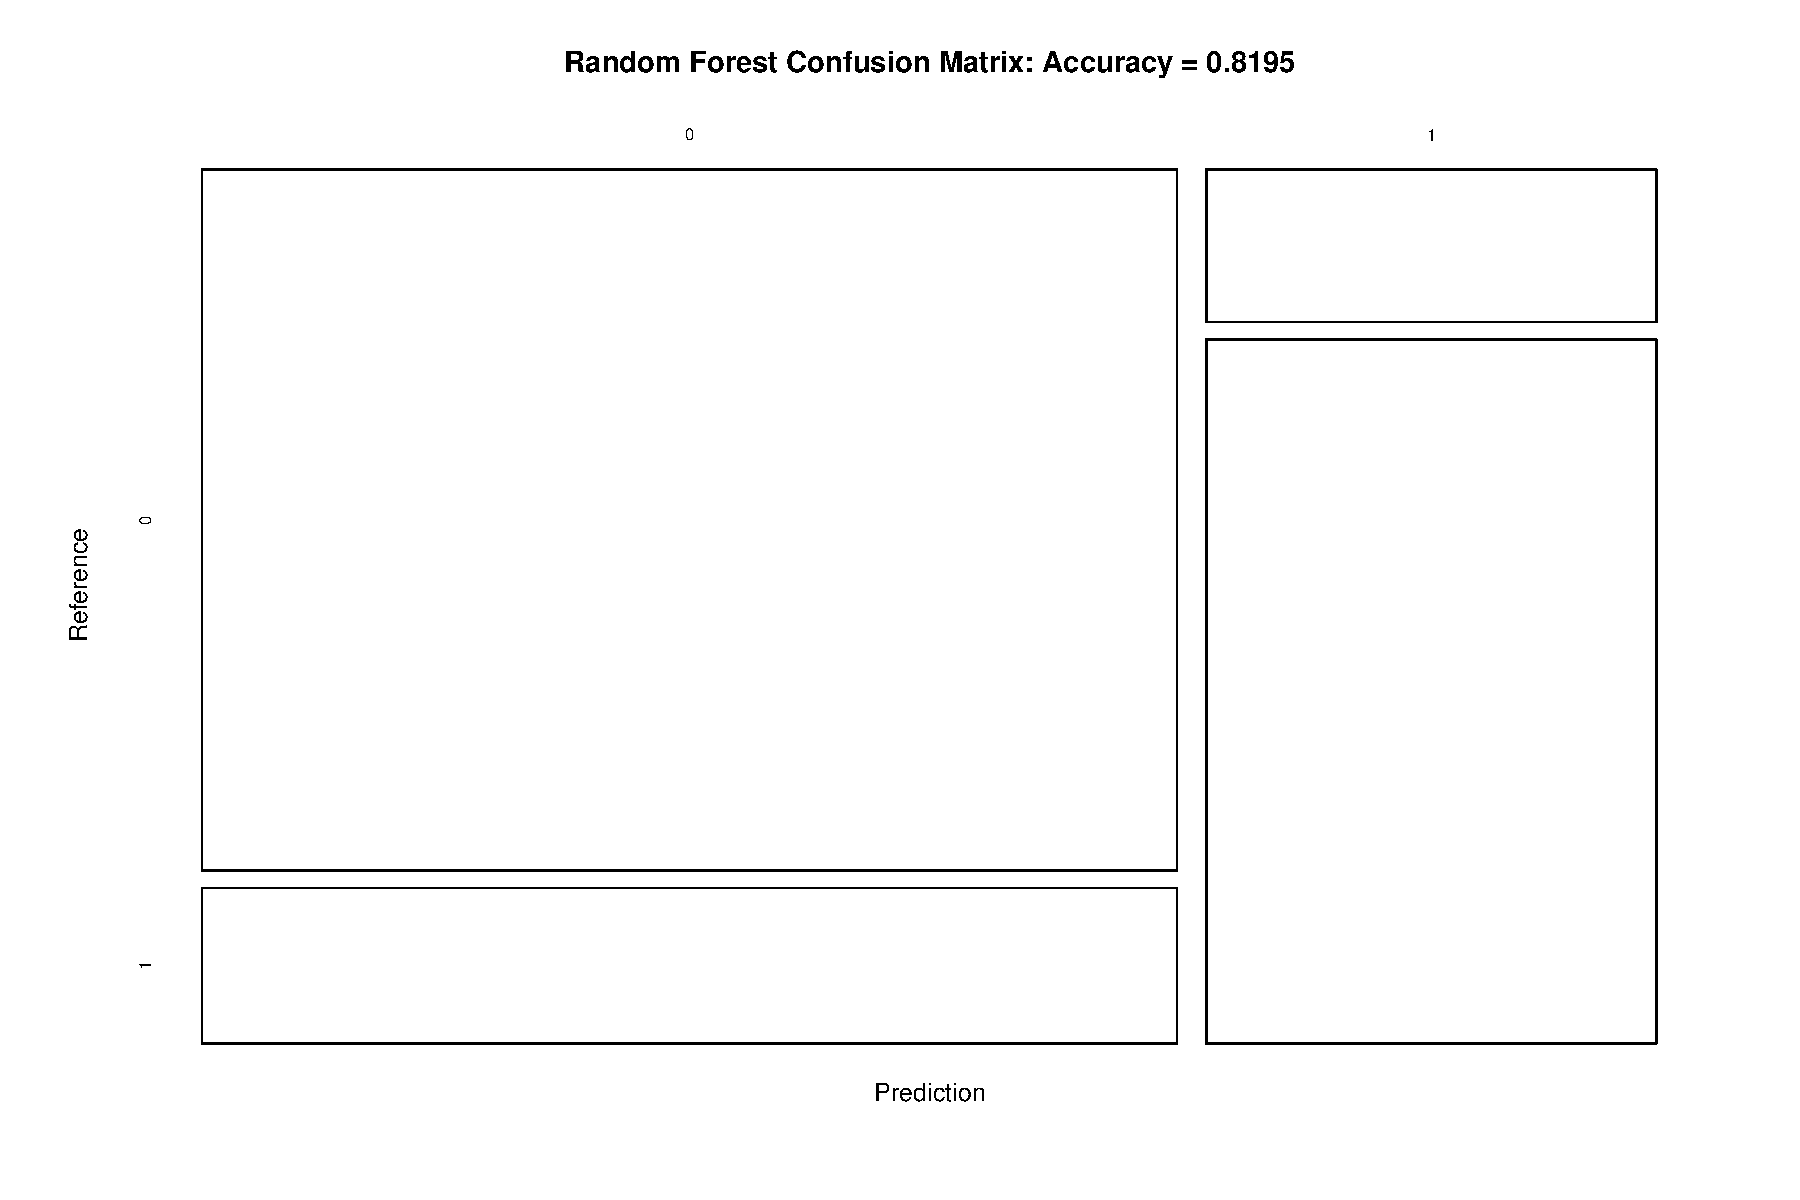
\includegraphics{figure/unnamed-chunk-15-1.pdf}

\paragraph{Generalized boosted regression
prediction}\label{generalized-boosted-regression-prediction}

\begin{Shaded}
\begin{Highlighting}[]
\KeywordTok{set.seed}\NormalTok{(}\DecValTok{12345}\NormalTok{)}
\NormalTok{val_fitControl <-}\StringTok{ }\KeywordTok{trainControl}\NormalTok{(}\DataTypeTok{method =} \StringTok{"repeatedcv"}\NormalTok{, }\DataTypeTok{number =} \DecValTok{5}\NormalTok{, }\DataTypeTok{repeats =} \DecValTok{1}\NormalTok{)}
\NormalTok{val_gbmmodel <-}\StringTok{ }\KeywordTok{train}\NormalTok{(Survived ~}\StringTok{ }\NormalTok{Pclass +}\StringTok{ }\NormalTok{Sex +}\StringTok{ }\NormalTok{Age +}\StringTok{ }\NormalTok{Fare +}\StringTok{ }\NormalTok{Embarked +}\StringTok{ }\NormalTok{FamilySize, }\DataTypeTok{data =} \NormalTok{data_training.train, }\DataTypeTok{method =} \StringTok{"gbm"}\NormalTok{, }\DataTypeTok{trControl =} \NormalTok{val_fitControl, }\DataTypeTok{verbose =} \OtherTok{FALSE}\NormalTok{)}
\NormalTok{val_gbmmodel.predict <-}\StringTok{ }\KeywordTok{predict}\NormalTok{(val_gbmmodel, }\DataTypeTok{newdata =} \NormalTok{data_training.test)}
\NormalTok{val_gbmcm <-}\StringTok{ }\KeywordTok{confusionMatrix}\NormalTok{(val_gbmmodel.predict, data_training.test$Survived)}
\NormalTok{val_gbmcm}
\end{Highlighting}
\end{Shaded}

\begin{verbatim}
## Confusion Matrix and Statistics
## 
##           Reference
## Prediction   0   1
##          0 148  39
##          1  16  63
##                                           
##                Accuracy : 0.7932          
##                  95% CI : (0.7395, 0.8403)
##     No Information Rate : 0.6165          
##     P-Value [Acc > NIR] : 4.694e-10       
##                                           
##                   Kappa : 0.5432          
##  Mcnemar's Test P-Value : 0.003012        
##                                           
##             Sensitivity : 0.9024          
##             Specificity : 0.6176          
##          Pos Pred Value : 0.7914          
##          Neg Pred Value : 0.7975          
##              Prevalence : 0.6165          
##          Detection Rate : 0.5564          
##    Detection Prevalence : 0.7030          
##       Balanced Accuracy : 0.7600          
##                                           
##        'Positive' Class : 0               
## 
\end{verbatim}

Generalized boosted regression prediction has a reported accuracy
against the training dataset:

\begin{Shaded}
\begin{Highlighting}[]
\KeywordTok{round}\NormalTok{(val_gbmcm$overall[}\StringTok{'Accuracy'}\NormalTok{], }\DecValTok{4}\NormalTok{)}
\end{Highlighting}
\end{Shaded}

\begin{verbatim}
## Accuracy 
##   0.7932
\end{verbatim}

\begin{Shaded}
\begin{Highlighting}[]
\KeywordTok{plot}\NormalTok{(val_gbmcm$table, }
     \DataTypeTok{col =} \NormalTok{val_gbmcm$byClass,}
     \DataTypeTok{main =} \KeywordTok{paste}\NormalTok{(}\StringTok{"Generalized Boosted Regression Confusion Matrix: Accuracy ="}\NormalTok{,}
     \KeywordTok{round}\NormalTok{(val_gbmcm$overall[}\StringTok{'Accuracy'}\NormalTok{], }\DecValTok{4}\NormalTok{)))}
\end{Highlighting}
\end{Shaded}

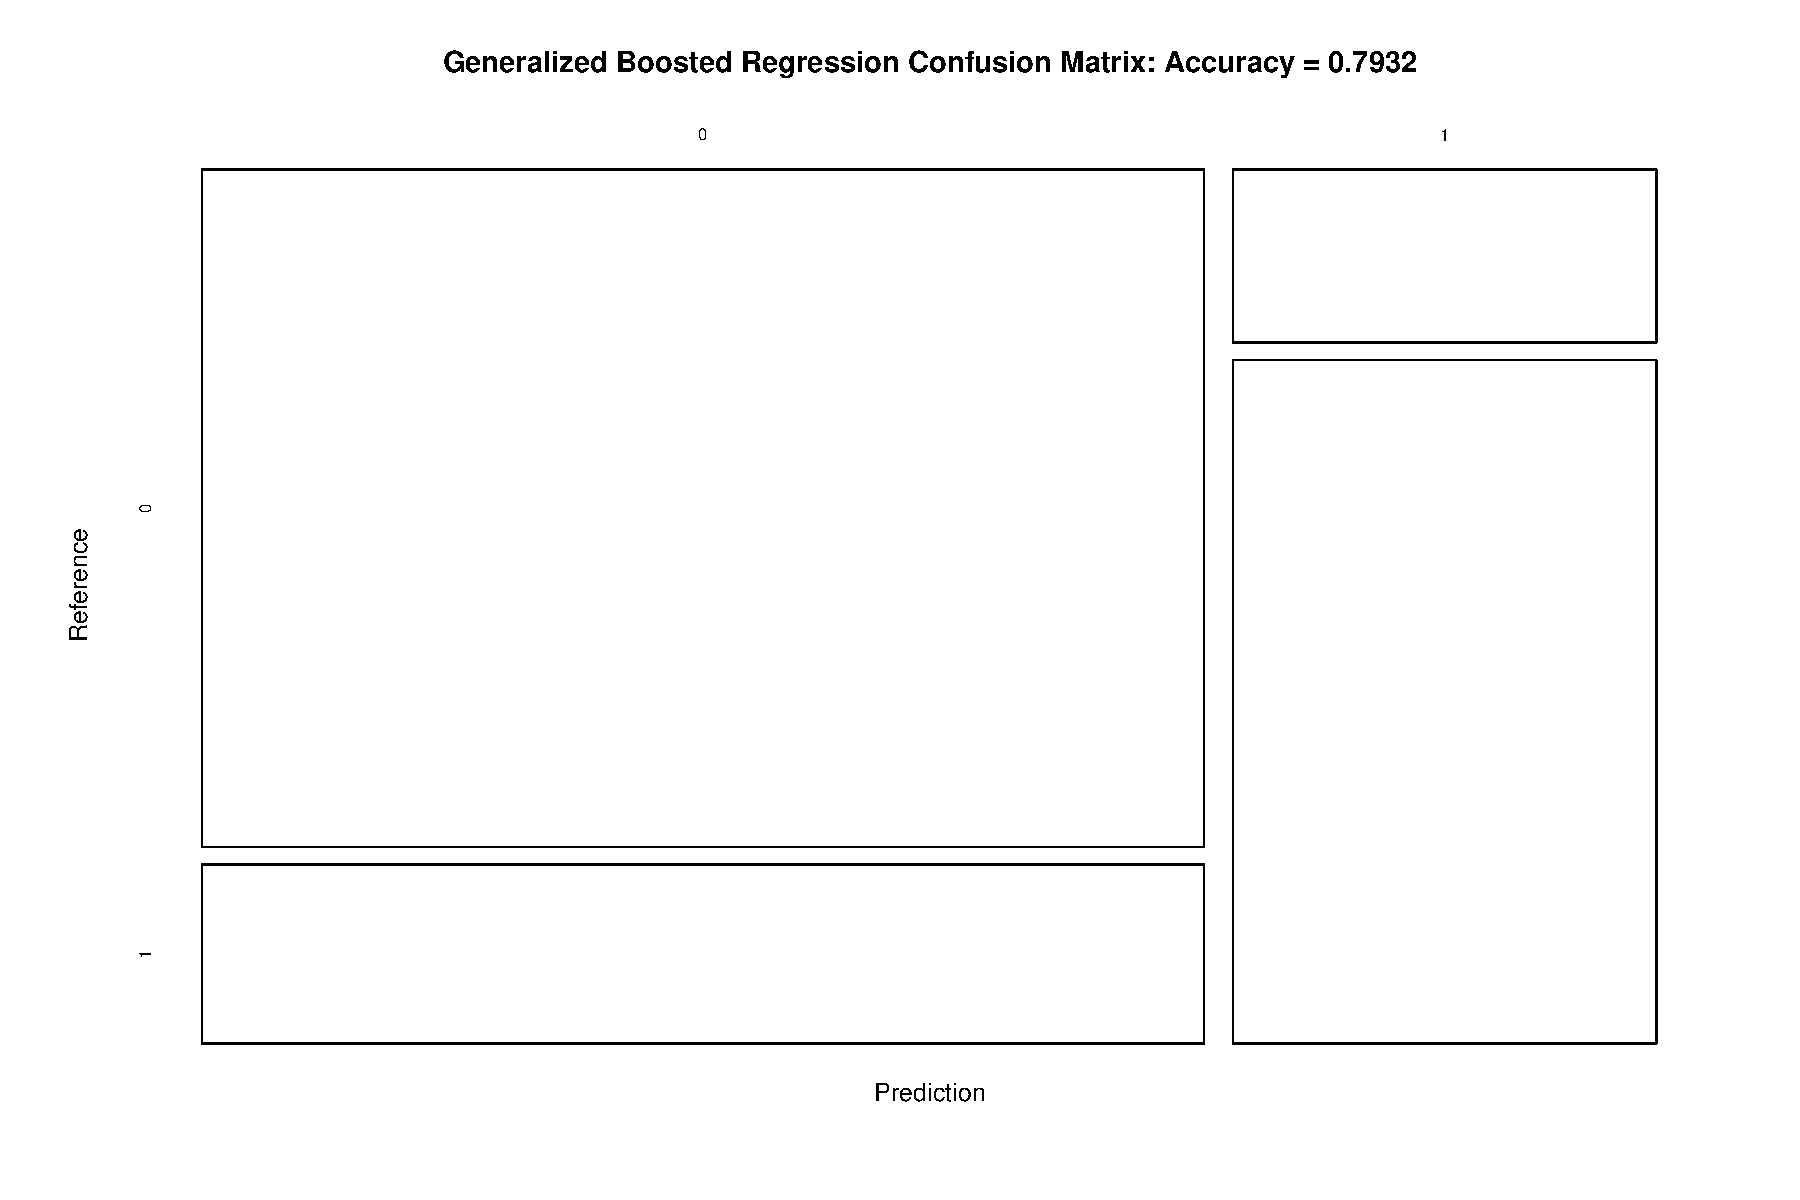
\includegraphics{figure/unnamed-chunk-18-1.pdf}

\subsubsection{4. Model Selection}\label{model-selection}

The expected out-of-sample error is calculated as 1 - accuracy for
predictions made against the cross-validation set:

\begin{Shaded}
\begin{Highlighting}[]
\NormalTok{val_ooserror <-}\StringTok{ }\DecValTok{1} \NormalTok{-}\StringTok{ }\KeywordTok{round}\NormalTok{(val_rfcm$overall[}\StringTok{'Accuracy'}\NormalTok{], }\DecValTok{4}\NormalTok{)}
\NormalTok{## val_ooserror <- 1 - round(val_gbmcm$overall['Accuracy'], 4)}
\NormalTok{val_ooserror}
\end{Highlighting}
\end{Shaded}

\begin{verbatim}
## Accuracy 
##   0.1805
\end{verbatim}

\begin{Shaded}
\begin{Highlighting}[]
\NormalTok{val_selmodel.final <-}\StringTok{ }\KeywordTok{predict}\NormalTok{(val_rfmodel, data_testing)}
\NormalTok{## val_selmodel.final <- predict(val_gbmmodel, data_testing)}
\end{Highlighting}
\end{Shaded}

\subsubsection{5. Kaggle Submission}\label{kaggle-submission}

\begin{Shaded}
\begin{Highlighting}[]
\NormalTok{data_prediction <-}\StringTok{ }\KeywordTok{data.frame}\NormalTok{(}\DataTypeTok{PassengerId =} \NormalTok{data_testing$PassengerId, }\DataTypeTok{Survived =} \NormalTok{val_selmodel.final)}
\KeywordTok{write.table}\NormalTok{(data_prediction,}\StringTok{"data/prediction.csv"}\NormalTok{, }\DataTypeTok{row.names =} \OtherTok{FALSE}\NormalTok{, }\DataTypeTok{sep=}\StringTok{","}\NormalTok{, }\DataTypeTok{col.names =} \OtherTok{TRUE}\NormalTok{)}
\end{Highlighting}
\end{Shaded}

\end{document}
